% ======================================================================
%  CleanWhite -- a sober, all-white Beamer template
%  Compile with pdflatex or lualatex (run TWICE for corner logos)
% ======================================================================
\documentclass[aspectratio=169,10pt]{beamer}

% ------------------------- PACKAGES -----------------------------------
\usepackage[T1]{fontenc}
\usepackage[utf8]{inputenc} % not needed on LuaLaTeX/XeLaTeX
\usepackage{lmodern}
\usepackage{graphicx}
\usepackage{booktabs}                 % clean tables
\usepackage{tikz}
\usepackage{pgfplots}
\graphicspath{{../Figures/}}
\pgfplotsset{compat=1.17}

% ======================================================================
%  EDIT ME -- presentation metadata & branding
% ======================================================================
\title[Short Title]{Full Presentation Title Goes Here}
\subtitle[Short Subtitle]{A Very Interesting and Precise Subtitle}
\author[Doe \& Smith]{Jane Doe, John Smith}
\date[09.09.2026]{September 9, 2026}

\newcommand{\ProjectName}{My Awesome Project}   % shown in footer
\newcommand{\AccentColor}{blue!65!black}        % try e.g. teal!70!black

%confidential
\newif\ifconfidential
\confidentialtrue   % set to \confidentialfalse or \confidentialfalse

% Corner logos (replace file names; or set \showcornerlogosfalse)
\newif\ifshowcornerlogos
\showcornerlogostrue 
\newcommand{\LogoTopRight}{
\includegraphics[height=0.95cm]{IE_HEIG-VD_logotype_rouge_rvb}}
\newcommand{\LogoBottomLeft}{
\includegraphics[height=2cm]{HES_SO_Logo_RGB}}

% ======================================================================
%  THEME: all white, hairlines only, one accent color
% ======================================================================
\definecolor{accent}{RGB}{225,37,27}
\definecolor{accenthesso}{RGB}{0,96,156}
\definecolor{textgrey}{RGB}{150,139,131}

\setbeamercolor{background canvas}{bg=white}
\setbeamercolor{normal text}{fg=black!87}
\setbeamercolor{structure}{fg=black!87}
\setbeamercolor{alerted text}{fg=accent}
\setbeamercolor{frametitle}{fg=accent}
\setbeamercolor{framesubtitle}{fg=textgrey}
\setbeamercolor{title}{fg=accent}
\setbeamercolor{subtitle}{fg=textgrey}
\setbeamercolor{author}{fg=textgrey}
\setbeamercolor{date}{fg=textgrey}
\setbeamercolor{item}{fg=black!87}
\setbeamercolor{enumerate item}{fg=accent!80}
\setbeamercolor{block title}{fg=black!87,bg=white}
\setbeamercolor{block body}{fg=black!80,bg=white}
\setbeamercolor{caption}{fg=textgrey}

\setbeamerfont{frametitle}{size=\large,series=\bfseries}
\setbeamerfont{framesubtitle}{size=\footnotesize}
\setbeamerfont{caption}{size=\footnotesize}
\setbeamerfont{block title}{size=\normalsize,series=\bfseries}

\setbeamertemplate{navigation symbols}{}
\setbeamersize{text margin left=3.1cm, text margin right=1.2cm}

% ---------- Frame titles (thin hairline under the title) --------------
\makeatletter
\setbeamertemplate{frametitle}{% 
  \vspace*{-0.3ex}%
  {\color{accent!60}\rule{0.33\linewidth}{0.5pt}}%$$
  \par\vspace*{-0.3ex}%
  {\usebeamercolor[fg]{frametitle}\usebeamerfont{frametitle}\insertframetitle}%

  \ifx
    %\par\vspace{-0.1em}%
    \insertframesubtitle\@empty%
  \else%
    \par\vspace{-0.3em}%
    {\usebeamercolor[fg]{framesubtitle}\usebeamerfont{framesubtitle}\insertframesubtitle}%
    \par\vspace{-0.7em}%
  \fi%

  {\color{accent!60}\rule{0.66\linewidth}{0.5pt}}%
  \par\vspace{0.1em}%
}
\makeatother

% ---------- Footline: title - subtitle - project - authors - date -----
\setbeamertemplate{footline}{%
  \leavevmode%
  \hbox{%
    \hspace*{40ex}%
    {\footnotesize\color{textgrey}%
      \insertshorttitle\;$\cdot$\;\insertshortsubtitle%
      \;$\cdot$\;\ProjectName%
      \;$\cdot$\;\insertshortauthor%
      \;$\cdot$\;\insertshortdate}%
    %\hfill%
    %{\scriptsize\color{black!75}\insertframenumber\,/\,\inserttotalframenumber}%
    %\hspace*{1.6ex}%
  }%
  \vspace*{5.7ex}%
}

% ---------- Corner logos (background canvas) ---------------------------

\makeatletter
\addtobeamertemplate{background canvas}{}{%
  % Corner logos (unchanged)
  \ifshowcornerlogos
    \begin{tikzpicture}[remember picture,overlay]
      \node[anchor=north west,inner sep=0pt]
        at ([yshift=-0.41cm,xshift=0.39cm]current page.north west) {\LogoTopRight};
      \node[anchor=south west,inner sep=0pt]
        at ([yshift=-0.3cm,xshift=-0.19cm]current page.south west) {\LogoBottomLeft};
    \end{tikzpicture}%
  \fi
  % Page number pinned to the bottom-right corner
  \ifbeamer@plainframe\else
    \begin{tikzpicture}[remember picture,overlay]
      \node[anchor=south east]
        at ([xshift=-0.55cm,yshift=0.4cm]current page.south east)
        {\footnotesize\color{textgrey}\insertframenumber};
    \end{tikzpicture}%
  \fi
  % --- CONFIDENTIAL stamp ---
  \ifconfidential
    \begin{tikzpicture}[remember picture,overlay]
      \node[anchor=north west, inner sep=0pt]
        at ([xshift=0.32cm,yshift=-1.6cm]current page.north west)
        {\footnotesize\sffamily\bfseries\color{accent}
         \setlength{\fboxsep}{2pt}%
         \fbox{\;CONFIDENTIAL\;}};
    \end{tikzpicture}%
  \fi
}
\makeatother

% ---------- Subtle bullets ---------------------------------------------
\setbeamertemplate{itemize item}{\textcolor{accent!75}{\footnotesize$\bullet$}}
\setbeamertemplate{itemize subitem}{\textcolor{accent!60}{\footnotesize--}}
\setbeamertemplate{itemize subsubitem}{\textcolor{textgrey}{\tiny$\bullet$}}
\setbeamertemplate{enumerate item}{\textcolor{accent!80}{\footnotesize\arabic{enumi}.}}

% ---------- Custom title page ------------------------------------------

\setbeamertemplate{title page}{%
  \begin{tikzpicture}[remember picture,overlay]
    \node[anchor=center, align=center, text width=0.85\paperwidth]
      at (current page.center) {%
        {\usebeamerfont{frametitle}\huge\bfseries\color{accent}\inserttitle\par}
        \vspace{0.45em}
        {\Large\color{textgrey}\insertsubtitle\par}
        \vspace{1.4em}
        {\color{accent!60}\rule{0.3\linewidth}{0.6pt}\par}
        \vspace{1.2em}
        {\insertauthor\par}
        \vspace{0.3em}
        {\small\color{textgrey}\ProjectName\par}
        \vspace{0.3em}
        {\small\color{textgrey}\insertdate\par}%
      };
  \end{tikzpicture}%
}

% ======================================================================
%  DOCUMENT
% ======================================================================
\begin{document}

% ------- Title page ----------------------------------------------------

\begin{frame}[plain]
  \titlepage
\end{frame}

% ------- Outline --------------------------------------------------------
\begin{frame}{Outline}
  \tableofcontents[hideallsubsections]
\end{frame}

% ------- Bullets ---------------------------------------------------------
\section{Motivation}
\begin{frame}{Why another template?}{Clean, sober, distraction-free}
  \begin{itemize}
    \item All-white background, single accent colors
    \item Unobtrusive bullets and hairline separators
    \item Logos in the corners, discreet footer
      \begin{itemize}
        \item Sub-items become quiet dashes
        \item Easy to extend with your own commands
      \end{itemize}
    \item Works with figures, tables and charts
  \end{itemize}
\end{frame}

% ------- Table -----------------------------------------------------------
\section{Results}
\begin{frame}{Example table}{Measured throughput (Mbit/s)}
  \begin{table}
    \centering
    \begin{tabular}{lccc}
      \toprule
      \textcolor{accent}{\textbf{Scheme}} &
      \textcolor{accent}{\textbf{Load A}} &
      \textcolor{accent}{\textbf{Load B}} &
      \textcolor{accenthesso}{\textbf{Gain}} \\
      \midrule
      Baseline      & 410 & 380 & --- \\
      Proposed      & 512 & 495 & +25\,\% \\
      Proposed + X  & 548 & 520 & +34\,\% \\
      \bottomrule
    \end{tabular}
  \end{table}
\end{frame}

% ------- Chart (native pgfplots) ------------------------------------------
\begin{frame}{Example chart with TIKZpicture}{Throughput over time}
  \begin{figure}
    \centering
    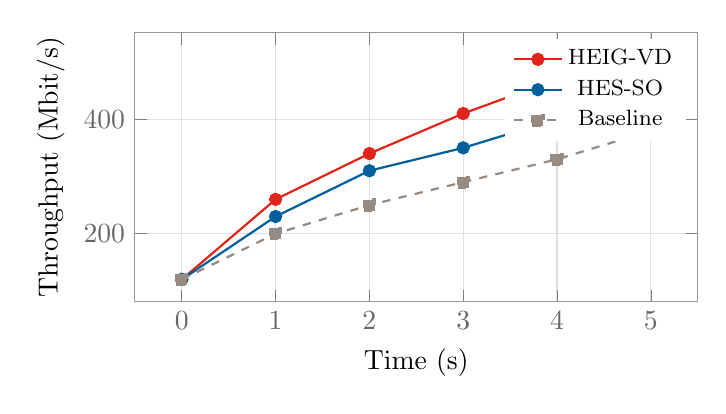
\begin{tikzpicture}
      \begin{axis}[
          width=0.72\linewidth, height=5cm,
          xlabel={Time (s)}, ylabel={Throughput (Mbit/s)},
          grid=major, grid style={black!12},
          axis line style={black!40}, tick label style={black!60},
          legend style={draw=none, font=\footnotesize},
        ]
        \addplot[accent, thick, mark=*] coordinates
          {(0,120)(1,260)(2,340)(3,410)(4,470)(5,512)};
          \addplot[accenthesso, thick, mark=*] coordinates
          {(0,120)(1,230)(2,310)(3,350)(4,400)(5,450)};
        \addplot[textgrey, thick, dashed, mark=square*] coordinates
          {(0,120)(1,200)(2,250)(3,290)(4,330)(5,380)};
        \legend{HEIG-VD, HES-SO, Baseline}
      \end{axis}
    \end{tikzpicture}
    \caption{Proposed scheme versus baseline.}
  \end{figure}
\end{frame}

% ------- External figure --------------------------------------------------
\begin{frame}{External figure}{Replace with your own graphic}
  \begin{figure}
    \centering
    \includegraphics[width=0.55\linewidth]{example-image-a}
  \end{figure}
\end{frame}

% ------- Columns ----------------------------------------------------------

\begin{frame}{Setup}{Experiment and results side by side}
  \begin{columns}[totalwidth=\textwidth]
    \begin{column}{0.5\textwidth}
      \textbf{Method}
      \begin{itemize}
        \item First condition
        \item Second condition
      \end{itemize}
    \end{column}
    \begin{column}{0.5\textwidth}
      \begin{figure}
        \includegraphics[width=\linewidth]{example-image-a}
        \caption{Result of the run.}
      \end{figure}
    \end{column}
  \end{columns}
\end{frame}

% ------- Blocks ------------------------------------------------------------
\section{Discussion}
\begin{frame}{Blocks are quiet too}
  \begin{block}{Key observation}
    Block titles are tinted light grey; bodies stay white.
  \end{block}
  \begin{alertblock}{Attention}
    Alerted blocks reuse the Master accent color.
  \end{alertblock}
\end{frame}

\end{document}